\documentclass[class={IEEEtran}]{standalone}
\usepackage{tikz}

\pagestyle{empty}
\usetikzlibrary{shapes.geometric,shapes.arrows,positioning,calc,arrows.meta,math}

\tikzset{ARROW/.style={thick, -stealth}}
\tikzset{ORACLE/.style={rectangle, minimum width=20em, minimum height=14.5ex, draw, semithick, align=flush left, anchor=north east}}

\linespread{1.25}

\begin{document}
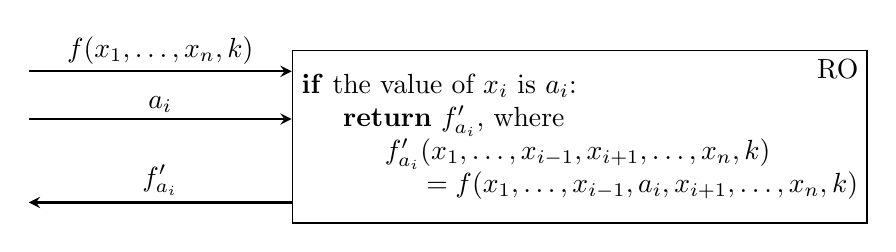
\begin{tikzpicture}
    \node[ORACLE] (n_oracle) {
        \hspace{0em}\textbf{if} the value of $x_i$ is $a_i$: \\
        \hspace{1.5em}\textbf{return} $f'_{a_i}$, where \\
        \hspace{3em}$f'_{a_i}(x_1, \ldots, x_{i-1}, x_{i+1}, \ldots, x_n, k)$ \\
        \hspace{4.5em}$= f(x_1, \ldots, x_{i-1}, a_i, x_{i+1}, \ldots, x_n, k)$
    };
    \node[anchor=north east] at (n_oracle.north east) {RO};

    \coordinate (input1) at ($(n_oracle.west)+(-9.5em, 5.5ex)$);
    \coordinate (input1_end) at ($(input1-|n_oracle.west)$);
    \draw[ARROW] (input1) -- (input1_end) node[midway,above=-0.3ex]{$f(x_1, \ldots, x_n, k)$};

    \coordinate (input2) at ($(n_oracle.west)+(-9.5em, 1.5ex)$);
    \coordinate (input2_end) at ($(input2-|n_oracle.west)$);
    \draw[ARROW] (input2) -- (input2_end) node[midway,above=-0.3ex]{$a_i$};

    \coordinate (output) at ($(n_oracle.west)+(-9.5em, -5.5ex)$);
    \coordinate (output_end) at ($(output-|n_oracle.west)$);
    \draw[ARROW] (output_end) -- (output) node[midway,above=-0.3ex]{$f'_{a_i}$};


\end{tikzpicture}

\end{document}
